\documentclass[border=10pt]{standalone}

\usepackage{tikz}
\usepackage{tikzsymbols}
\usetikzlibrary{calc,patterns,shapes.geometric}

\def\centerarc[#1](#2)(#3:#4:#5){\draw[#1] ($(#2)+({#5*cos(#3)},{#5*sin(#3)})$) arc (#3:#4:#5);}

\begin{document}
	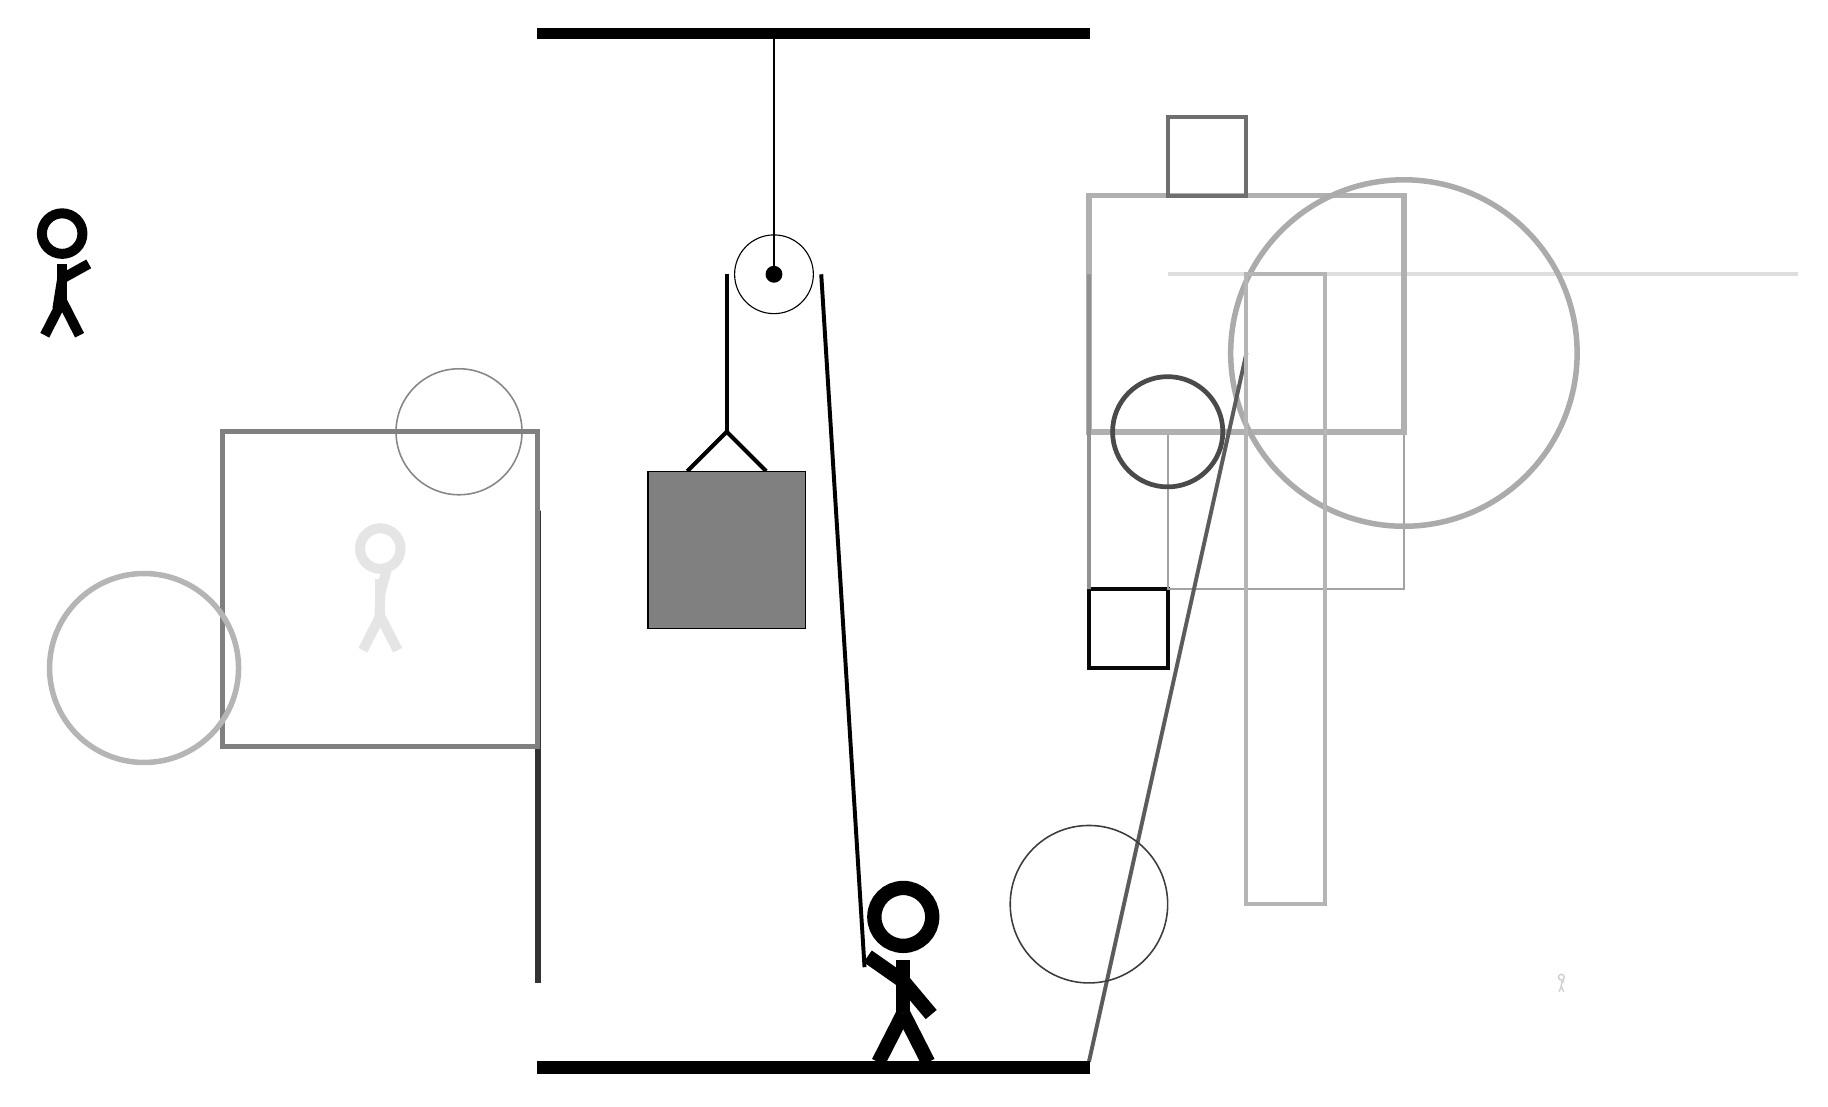
\begin{tikzpicture}
		%%%%% START %%%%%
		
		\draw[fill=black] (-2, 10) rectangle (5, 10.125);
		
		\draw (1, 7) circle (0.5);
		\draw[fill=black] (1, 7) circle (0.1);
		\draw (1, 10) -- (1, 7);
		
		\draw[line width=0.5mm] (-0.1, 4.5) -- (0.4, 5.0) -- (0.9, 4.5);
		\draw[fill=black!50] (-0.6, 4.5) rectangle (1.4, 2.5);
		
		\node[line width=0.5mm, color=black!10] at (-4, 3) {\Strichmaxerl[7][88][75]};
		
		\draw[line width=0.7mm, color=black!80] (-2, -2) rectangle (-2, 4);
		\draw[line width=0.5mm, color=black!97] (6, 3) rectangle (5, 2);
		\draw[line width=0.5mm, color=black!13](6, 7) -- (14, 7);
		
		\node[line width=0.5mm, color=black!99] at (-8, 7) {\Strichmaxerl[7][81][29]};
		\node[line width=0.7mm, color=black!19] at (11, -2) {\Strichmaxerl[1][87][50]};
		\draw[line width=0.3mm, color=black!36] (6, 5) rectangle (9, 3);
		\draw[line width=0.7mm, color=black!31] (5, 5) rectangle (9, 8);
		\draw [line width=0.6mm, color=black!71](6, 5) circle (0.7);
		\draw [line width=0.7mm, color=black!33](9, 6) circle (2.2);
		\draw[line width=0.5mm, color=black!64](5, -3) -- (7, 6);
		\draw [line width=0.2mm, color=black!47](-3, 5) circle (0.8);
		\draw[line width=0.6mm, color=black!50] (-2, 1) rectangle (-6, 5);
		\draw[line width=0.5mm, color=black!57] (6, 8) rectangle (7, 9);
		\draw [line width=0.2mm, color=black!76](5, -1) circle (1.0);
		\draw [line width=0.7mm, color=black!29](-7, 2) circle (1.2);
		
		\draw[line width=0.5mm, color=black!29] (7, -1) rectangle (8, 7);
		
		\draw[line width=0.6mm, color=black!43] (5, 7) rectangle (5, 3);
		
		\draw[line width=0.5mm] (0.4, 7) -- (0.4, 5.0);
		\centerarc[line width=0.5mm](1, 7)(0:180:0.6);
		\draw[line width=0.5mm](1.6, 7) -- (2.15, -1.8);
		
		\node at (2.6, -1.9) {\Strichmaxerl[10][-35][-50]};
		
		\draw[fill=black] (-2, -3) rectangle (5, -3.15);
		
		%%%%% END %%%%%
	\end{tikzpicture}
\end{document}